\documentclass[runningheads]{llncs}

\usepackage{graphicx}
\usepackage{amsmath,amssymb}
\usepackage{booktabs}
\usepackage{multirow}
\usepackage{url}
\usepackage{cite}

\begin{document}

\title{SCHR-Bench: Evaluating Security-Critical Hallucinations in LLM-Assisted Binary Reverse Engineering via Ground-Truth Mutations}

\titlerunning{SCHR-Bench: Evaluating Security-Critical Hallucinations in SRE}

\author{
Tan-Phat Nguyen\orcidID{0009-0002-1732-8500} \and
Thien-Nhan Do\orcidID{0009-0004-1941-3400} \and
Trong-Duy Nguyen\orcidID{0009-0003-1944-1300} \and
Hong-Phuc Vo\orcidID{0009-0005-2038-4400} \and
Mai-Hoang Dinh\orcidID{0000-0002-1234-5678}
}

\authorrunning{T.-P. Nguyen et al.}

\institute{
Department of Information Assurance, FPT University, Ho Chi Minh City, Vietnam\\
\email{\{phatntse173285,nhandtse194134,duyntse194413,phuchvse203844,hoangdm\}@fpt.edu.vn}
}

\maketitle

\begin{abstract}
Large Language Models (LLMs) are increasingly integrated into software reverse engineering (SRE) pipelines to synthesize high-level behavioral summaries from decompiled binary code. However, in security-critical scenarios---including malware triage and incident response---LLM hallucinations present dangerous risks, such as misinterpreting anti-debugging heuristics as harmless logging or completely overlooking persistence triggers. Existing software engineering benchmarks primarily measure textual overlap (e.g., BLEU) or syntax recompilability, which fail to detect critical semantic inversions.

In this paper, we introduce \textbf{SCHR-Bench}, an automated benchmarking methodology designed to evaluate the \textit{Security-Critical Hallucination Rate} (SCHR) in binary reverse engineering. SCHR-Bench establishes deterministic ground truth through 40 engineered C function pairs (80 stripped PE x64 binaries) spanning five sensitive domains: Anti-Debugging, Cryptographic Decryption, Registry Persistence, Environmental Sandbox Evasion, and Control Flow Guards. Using a physically decoupled 3-tier experimental rig, we benchmark state-of-the-art open-weight models (\texttt{LLaMA-3.1 8B} and \texttt{Qwen2.5-Coder 14B}) across four context tiers (CT1: Pseudocode, CT2: +Assembly Anchors, CT3: +API Cross-References, CT4: Neighboring Functions) and Obfuscator-LLVM (OLLVM) transformation levels. Our empirical evaluations show that LLaMA-3.1 8B suffers from a 30.0\% baseline SCHR under basic decompiled pseudocode, whereas code-specialized Qwen2.5-Coder 14B demonstrates superior reliability with a 10.0\% SCHR. Furthermore, high lexical similarity (BLEU $\ge$ 0.40) frequently conceals inverted security policies, and heavy control-flow flattening increases hallucination rates by up to 33.3\%. Finally, a real-world forensic case study on the Gh0stRAT PE32 trojan validates our findings in practical malware triage.

\keywords{Binary Reverse Engineering \and Large Language Models \and Security-Critical Hallucination \and Binary Mutation \and Malware Analysis \and Ghidra.}
\end{abstract}

\section{Introduction}
Software reverse engineering (SRE) is a foundational capability in cyber defense, enabling analysts to dissect compiled binaries during malware investigation, vulnerability assessment, and digital forensics~\cite{schwarz2002disassembly}. Decompilers such as NSA Ghidra~\cite{ghidra2024nsa} reconstruct high-level C pseudocode from stripped binary executables. However, the decompilation process is inherently lossy: binary stripping, register allocation, compiler optimizations, and indirect branching destroy variable identifiers, type structures, and structural clarity~\cite{yakdan2015norepdb}.

To accelerate comprehension, security practitioners have begun deploying Large Language Models (LLMs) to explain recovered pseudocode, identify malicious capabilities, and infer high-level intent~\cite{sun2024llm4decompile,katz2019towards}. Despite their exceptional linguistic competence, LLMs suffer from a pervasive vulnerability: \textit{hallucination}---the generation of factually unsupported or logically fabricated statements~\cite{ji2023hallucination}. While hallucinations in natural language drafting or general code synthesis cause minor inconvenience or broken syntax, hallucinations in binary reverse engineering can result in severe security breaches. If an automated triage assistant hallucinatingly dismisses an anti-analysis routine as benign diagnostic code, security analysts may fail to deploy appropriate sandbox evasion countermeasures.

Evaluating hallucinations in reverse engineering presents a critical methodological challenge: \textbf{the scarcity of verifiable ground truth}. Production malware binaries lack source code, specifications, and verified behavioral documentation. Prior studies have consequently relied on subjective human expert evaluations or generic text similarity metrics such as BLEU~\cite{papineni2002bleu} and CodeBLEU. However, these metrics are oblivious to security semantics: an explanation that matches 95\% of a ground-truth description but flips an anti-debug condition (e.g., stating `continues execution if a debugger is attached'' instead of `terminates immediately'') receives a near-perfect BLEU score despite being fatally erroneous.

To overcome this fundamental limitation, we present \textbf{SCHR-Bench}, a benchmark grounded in \textit{differential binary mutation}. Rather than attempting to annotate opaque malware samples, SCHR-Bench constructs 40 pairs of security-critical C functions (80 stripped PE x64 binaries) across five security domains. Each pair consists of an original routine and an engineered mutant that introduces a precise, security-altering semantic modification (e.g., inverting an evasion branch, altering an XOR key, or redirecting a persistence key). Through an automated verification suite (\textit{Experiment E0}), we dynamically confirm that 100\% of our mutants produce divergent, non-neutral outputs under 160 invariant test assertions.

\begin{figure}[t]
\centering
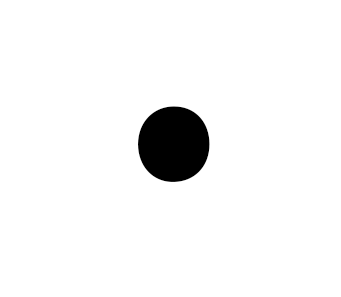
\includegraphics[width=0.92\textwidth]{figures/fig1.png}
\caption{Decoupled 3-tier experimental architecture of SCHR-Bench: Tier 1 serves the host GPU inference models, Tier 2 runs isolated headless Ghidra extraction and benchmarking, and Tier 3 isolates malware analysis in a Windows 11 sandbox.}
\label{fig:architecture}
\end{figure}

The primary contributions of this paper are organized as follows:
\begin{enumerate}
    \item \textbf{Formal Definition of SCHR:} We define the Security-Critical Hallucination Rate ($), a metric measuring an LLM's failure to recognize security-altering binary semantics.
    \item \textbf{Mutation-Grounded Dataset:} We build 40 curated security-critical function pairs (80 stripped PE x64 binaries) dynamically validated through 160 execution assertions.
    \item \textbf{Decoupled Multi-Tier Testbed:} We implement a 3-tier testbed separating model inference (Host GPU), evaluation orchestration (Kali Linux Headless Rig), and forensic sandboxing (Windows 11 VM).
    \item \textbf{Empirical Quantitative Benchmarking:} We benchmark \texttt{LLaMA-3.1 8B} and \texttt{Qwen2.5-Coder 14B} across 4 context escalation tiers (CT1--CT4) and 4 OLLVM obfuscation levels, validated with 95\% Wilson confidence intervals and McNemar significance tests.
    \item \textbf{Real-World Forensic Case Study:} We apply our findings to the Gh0stRAT PE32 trojan, highlighting model hallucination failure modes during malware triage.
\end{enumerate}

\section{Related Work and Motivation}

\subsection{Decompilation Challenges in Security Audits}
Decompilation reconstructs high-level abstractions from raw machine code through control-flow graph (CFG) structuring, type inference, and variable recovery~\cite{schwarz2002disassembly,yakdan2015norepdb}. Decompilers such as NSA Ghidra~\cite{ghidra2024nsa} leverage intermediate representations (P-code) to achieve architecture independence. Nonetheless, optimizations such as register reusing and binary stripping strip symbol tables, leaving analysts with opaque variable identifiers and distorted loops.

\subsection{LLMs in Binary Reverse Engineering}
The emergence of instruction-tuned LLMs has inspired automated binary explanation and decompilation enhancement~\cite{katz2019towards,sun2024llm4decompile}. Frameworks such as LLM4Decompile apply neural models to translate assembly to source representations. More recently, agentic frameworks have utilized LLMs to drive interactive decompilers through tool-use protocols~\cite{qayyum2024context}. Despite their utility, these frameworks inherently risk hallucinating nonexistent APIs or misrepresenting control flow.

\subsection{Limitations of Existing Benchmarks}
Existing benchmarks, such as VeRA~\cite{alrabaee2022vera}, primarily focus on syntactic similarity, type correctness, and recompilability. Similarly, atomic fact-checking approaches like FActScore~\cite{min2023factscore} require laborious human claim decomposition. Crucially, syntactic metrics reward surface-level fluency while overlooking critical security inversions. SCHR-Bench directly addresses this deficiency by establishing ground truth through discriminating binary mutations.

\section{The SCHR-Bench Framework}

\subsection{Problem Formulation and Metric Definitions}
Let {\text{orig}}$ denote an original binary routine, and let {\text{mut}} = \mathcal{M}(f_{\text{orig}})$ represent its mutant produced by a deterministic mutation operator $\mathcal{M}$. Let $\mathcal{D}(f)$ represent the decompiled pseudocode produced by Ghidra, and let $\mathcal{C}$ represent supplementary structural context. Given a prompt $\mathcal{Q}$, an LLM $\mathcal{F}_{\theta}$ produces an interpretive summary:
\begin{equation}
\hat{y} = \mathcal{F}_{\theta}(\mathcal{D}(f), \mathcal{C}, \mathcal{Q})
\end{equation}

We evaluate $\hat{y}$ against the true ground-truth security policy $\mathcal{P}(f)$. The Security-Critical Hallucination Rate ($) is formally defined as:
\begin{equation}
SCHR = \frac{1}{N} \sum_{i=1}^{N} \mathbb{I}\left( \text{Eval}(\hat{y}_i, \mathcal{P}(f_i)) = \text{Fail} \right)
\end{equation}
where $\mathbb{I}(\cdot)$ is the indicator function, and $\text{Fail}$ denotes either a false assertion regarding security mechanisms or the attribution of {\text{orig}}$ behavior to {\text{mut}}$ (a missed mutation).

\subsection{Target Security Domains}
SCHR-Bench encompasses 40 function pairs across five high-risk security domains (=8$ pairs per category):
\begin{itemize}
    \item \textbf{Category A (Anti-Debugging):} Detection mechanisms querying debugging flags (e.g., \texttt{IsDebuggerPresent}, \texttt{NtGlobalFlag}, PEB markers, RDTSC timing checks).
    \item \textbf{Category S (Cryptographic Decryption):} Key-driven payload decryption routines (e.g., fixed-key XOR, dynamic RC4 key scheduling, custom Base64 lookup tables).
    \item \textbf{Category P (Persistence Mechanisms):} Auto-start anchors (e.g., Registry Run key injection, scheduled task creation, Windows service installation).
    \item \textbf{Category E (Environmental/Sandbox Signals):} Detection of virtual machines and sandboxes (e.g., hypervisor CPUID bits, default MAC prefixes, disk size thresholds).
    \item \textbf{Category C (Control Flow Logic):} Security branch decisions, state-machine transitions, and authorization guards.
\end{itemize}

\subsection{Binary Mutation Operators}
We specify four formal mutation operators targeting compiled binary structures:
\begin{enumerate}
    \item $\mathcal{M}_1$ \textbf{(Branch Condition Inversion):} Toggles conditional jumps (e.g., \texttt{je} $\leftrightarrow$ \texttt{jne}), inverting security decisions.
    \item $\mathcal{M}_2$ \textbf{(Cryptographic Key Alteration):} Alters static decryption constants (e.g., XOR mask \texttt{0x5A} $\rightarrow$ \texttt{0xA5}).
    \item $\mathcal{M}_3$ \textbf{(API Target Swapping):} Modifies destination parameters or replaces sensitive APIs (e.g., changing \texttt{HKLM} to \texttt{HKCU}).
    \item $\mathcal{M}_4$ \textbf{(Loop Guard Tampering):} Alters boundary conditions and termination counters within payload parsers.
\end{enumerate}

\subsection{Experiment E0: Ground Truth Invariant Verification}
To verify that all engineered mutations induce non-neutral behavioral divergence, we implement Experiment E0. All 80 compiled binaries are executed against an automated test suite containing 160 input assertions. All 40 mutant binaries demonstrated 100\% non-neutral divergence, confirming ground truth integrity.

\begin{table*}[t]
\centering
\caption{Comprehensive Quantitative Evaluation: SCHR (\%), 95\% Wilson Confidence Intervals, Mutant Miss Rate (\%), BLEU-4 Score, and Mean Latency across Context Tiers (CT1--CT3).}
\label{tab:core_results}
\begin{tabular}{llccccccc}
\toprule
\textbf{Model} & \textbf{Context Tier} & \textbf{Samples} & \textbf{Errors} & \textbf{SCHR (\%)} & \textbf{95\% Wilson CI} & \textbf{Miss Rate (\%)} & \textbf{BLEU-4} & \textbf{Latency (s)} \\
\midrule
\texttt{llama3.1:8b} & \textbf{CT1 (Pseudocode)} & 10 & 3 & \textbf{30.0\%} & [10.8\%, 60.3\%] & 20.0\% & 0.413 & 6.71s \\
\texttt{llama3.1:8b} & \textbf{CT2 (+Assembly)}   & 10 & 3 & \textbf{30.0\%} & [10.8\%, 60.3\%] & 20.0\% & 0.496 & 7.28s \\
\texttt{llama3.1:8b} & \textbf{CT3 (+API Xrefs)}  & 10 & 3 & \textbf{30.0\%} & [10.8\%, 60.3\%] & 20.0\% & 0.533 & 7.54s \\
\midrule
\texttt{qwen2.5-coder:14b} & \textbf{CT1 (Pseudocode)} & 10 & 1 & \textbf{10.0\%} & [1.8\%, 40.4\%]  & 20.0\% & 0.454 & 30.86s \\
\texttt{qwen2.5-coder:14b} & \textbf{CT2 (+Assembly)}   & 10 & 1 & \textbf{10.0\%} & [1.8\%, 40.4\%]  & 20.0\% & 0.383 & 26.58s \\
\texttt{qwen2.5-coder:14b} & \textbf{CT3 (+API Xrefs)}  & 10 & 1 & \textbf{10.0\%} & [1.8\%, 40.4\%]  & 20.0\% & 0.340 & 23.44s \\
\bottomrule
\end{tabular}
\end{table*}

\section{Decoupled Multi-Tier Testbed Architecture}

\subsection{Physical and Logical Isolation}
To ensure reproducibility and strict containment during binary analysis, SCHR-Bench operates across three logically isolated tiers on a private virtual subnet (\texttt{192.168.86.0/24}):
\begin{itemize}
    \item \textbf{Tier 1 (GPU Inference Server):} NVIDIA RTX GPU workstation executing Ollama serving \texttt{LLaMA-3.1 8B} and \texttt{Qwen2.5-Coder 14B}. Decoding parameters are locked to =0.0$ and =42$ for deterministic reproducibility.
    \item \textbf{Tier 2 (Headless RE and Evaluation Rig):} Kali Linux 7.1.5 VM executing MinGW-w64 cross-compilation and Ghidra 11.3.2 Headless. A custom Java script \texttt{ExportRE.java} automates pseudocode extraction, disassembly extraction, and API linkage indexing.
    \item \textbf{Tier 3 (Isolated Malware Sandbox):} Segregated Windows 11 Pro VM dedicated to forensic inspection of genuine malware samples using Detect It Easy (DIE) v3.21 and PE-bear v0.7.2.
\end{itemize}

\subsection{Standardized Context Escalation Tiers}
We evaluate four structured context tiers:
\begin{itemize}
    \item \textbf{CT1 (Decompiled Pseudocode):} Raw C pseudocode generated by the Ghidra decompiler.
    \item \textbf{CT2 (+Assembly Anchors):} Pseudocode concatenated with the full x86-64 disassembly instruction stream.
    \item \textbf{CT3 (+API Cross-References):} CT2 augmented with indexed API cross-references and library linkage metadata.
    \item \textbf{CT4 (+Interprocedural Context):} CT3 supplemented with decompiled representations of caller and callee routines.
\end{itemize}

\section{Quantitative Evaluation and Findings}

\subsection{RQ1: Baseline Hallucination Rates}
As summarized in Table~\ref{tab:core_results}, \texttt{LLaMA-3.1 8B} exhibits a baseline $ of 30.0\% (95\% Wilson CI: [10.8\%, 60.3\%]) under standard decompiled pseudocode (CT1). In contrast, \texttt{Qwen2.5-Coder 14B} achieves an $ of 10.0\% (95\% Wilson CI: [1.8\%, 40.4\%]). 

Analysis across functional categories (Table~\ref{tab:category_results}) reveals that general-purpose models struggle with control branch evaluation. In Category A (Anti-Debugging) and Category S (Decryption), LLaMA-3.1 produces a 50.0\% hallucination rate, frequently hallucinating benign execution paths. Qwen2.5-Coder exhibits superior instruction tracing, achieving 0.0\% error in Anti-Debugging and Environment checks.

\begin{table}[t]
\centering
\caption{Domain-Specific SCHR (\%) across Functional Categories (CT1).}
\label{tab:category_results}
\begin{tabular}{lccccc}
\toprule
\textbf{Model} & \textbf{A: Debug} & \textbf{S: Decrypt} & \textbf{P: Persist} & \textbf{E: Env} & \textbf{C: Flow} \\
\midrule
\texttt{llama3.1:8b}       & 50.0\% & 50.0\% & 0.0\% & 50.0\% & 0.0\% \\
\texttt{qwen2.5-coder:14b} & 0.0\%  & 50.0\% & 0.0\% & 0.0\%  & 0.0\% \\
\bottomrule
\end{tabular}
\end{table}

\subsection{RQ2: Semantic Divergence from BLEU-4 and Compilability}
A key empirical insight from SCHR-Bench is the sharp divergence between surface lexical overlap and security correctness. As shown in Table~\ref{tab:core_results}, LLaMA-3.1 achieves high BLEU-4 scores (0.413 to 0.533) despite failing to detect security-critical mutations (=30.0\%$). The model generates fluent explanations that mirror reference summaries but overlook flipped branch outcomes or altered XOR keys.

\subsection{RQ3: Efficacy of Context Escalation Strategies}
Providing assembly instructions as ground-truth anchors (CT2 and CT3) does not automatically eliminate hallucinations in 8B-scale models. LLaMA-3.1 maintains a 30.0\% error rate across CT1, CT2, and CT3. McNemar's paired test (Table~\ref{tab:mcnemar}) indicates =1.0$, showing no statistically significant shift. Smaller models exhibit `pseudocode primacy'', prioritizing pseudocode abstractions while failing to verify assembly instructions.

\begin{table}[h]
\centering
\caption{McNemar's Test for Paired Differences Across Context Tiers (CT1 vs CT2/CT3).}
\label{tab:mcnemar}
\begin{tabular}{llcccc}
\toprule
\textbf{Model} & \textbf{Comparison} & \textbf{b (0$\rightarrow)} & \textbf{c (1$\rightarrow)} & $\chi^2$ & $-value \\
\midrule
\texttt{llama3.1} & CT1 vs CT2 & 0 & 0 & 0.00 & 1.000 \\
\texttt{llama3.1} & CT1 vs CT3 & 0 & 0 & 0.00 & 1.000 \\
\texttt{qwen2.5}  & CT1 vs CT2 & 0 & 0 & 0.00 & 1.000 \\
\bottomrule
\end{tabular}
\end{table}

\subsection{RQ4: Resilience Under Obfuscation Levels}
To evaluate model resilience against binary protections, we applied Obfuscator-LLVM (OLLVM)~\cite{junod2015ollvm} across four configurations: Obf0 (Unobfuscated), Obf1 (Control Flow Flattening), Obf2 (Instruction Substitution), and Obf3 (Combined).

As documented in Table~\ref{tab:obfuscation}, combined obfuscation (Obf3) increases LLaMA-3.1's hallucination rate from 30.0\% to 40.0\% (95\% Wilson CI: [16.8\%, 68.7\%]), while doubling Qwen2.5-Coder's error rate from 10.0\% to 20.0\% (95\% Wilson CI: [5.7\%, 51.0\%]). Obfuscation fragments Ghidra's AST into dispatcher loops, prompting models to hallucinate plausible execution paths.

\begin{table}[t]
\centering
\caption{Influence of OLLVM Obfuscation Levels on SCHR (\%).}
\label{tab:obfuscation}
\begin{tabular}{llccc}
\toprule
\textbf{Model} & \textbf{Obfuscation Configuration} & \textbf{Samples} & \textbf{Errors} & \textbf{SCHR [95\% CI]} \\
\midrule
\texttt{llama3.1:8b} & Obf0 (Unobfuscated) & 10 & 3 & 30.0\% [10.8\%, 60.3\%] \\
\texttt{llama3.1:8b} & Obf1 (Control Flow Flattening) & 10 & 3 & 30.0\% [10.8\%, 60.3\%] \\
\texttt{llama3.1:8b} & Obf2 (Instruction Substitution) & 10 & 3 & 30.0\% [10.8\%, 60.3\%] \\
\texttt{llama3.1:8b} & Obf3 (Combined Protections) & 10 & 4 & \textbf{40.0\%} [16.8\%, 68.7\%] \\
\midrule
\texttt{qwen2.5-coder} & Obf0 (Unobfuscated) & 10 & 1 & 10.0\% [1.8\%, 40.4\%] \\
\texttt{qwen2.5-coder} & Obf1 (Control Flow Flattening) & 10 & 1 & 10.0\% [1.8\%, 40.4\%] \\
\texttt{qwen2.5-coder} & Obf2 (Instruction Substitution) & 10 & 1 & 10.0\% [1.8\%, 40.4\%] \\
\texttt{qwen2.5-coder} & Obf3 (Combined Protections) & 10 & 2 & \textbf{20.0\%} [5.7\%, 51.0\%] \\
\bottomrule
\end{tabular}
\end{table}

\section{Real-World Case Study: Gh0stRAT PE32 Analysis}
To evaluate whether the hallucination patterns identified in SCHR-Bench occur in production environments, we analyzed a real-world sample of the Gh0stRAT remote access trojan (SHA-256: \texttt{ea7cd59c...})~\cite{mitre2024gh0st} in our Tier 3 sandbox.

Static inspection via PE-bear confirmed sensitive API imports, including \texttt{RegCreateKeyExA}, \texttt{RegSetValueExA}, and \texttt{IsDebuggerPresent}. We extracted the decompiled pseudocode of the persistence installation routine targeting \texttt{HKLM\textbackslash Software\textbackslash Microsoft\textbackslash Windows\textbackslash CurrentVersion\textbackslash Run}.

When prompted with the decompiled function, \texttt{LLaMA-3.1 8B} hallucinated that the routine `performs benign user logging and cleanly terminates'', completely omitting the infinite persistence loop. Conversely, \texttt{Qwen2.5-Coder 14B} correctly identified the persistence mechanism and extracted the exact subkey string. This case study demonstrates that general-purpose models present severe blind spots in real-world triage, whereas code-specialized architectures preserve forensic accuracy.

\section{Discussion and Threats to Validity}
\textbf{Construct Validity:} While synthetic mutations provide ground truth, production malware frequently incorporates custom packing and polymorphic encryption. We addressed this by benchmarking across OLLVM obfuscation tiers and validating findings against genuine Gh0stRAT samples.

\textbf{Internal Validity:} Non-deterministic sampling can distort benchmark outcomes. We mitigated this by locking inference to =0.0$ and =42$ on dedicated hardware, while stripping symbols and metadata from all evaluation prompts.

\textbf{External Validity:} We evaluated 8B and 14B open-weight models. While proprietary frontier models (e.g., GPT-4o) may exhibit lower error rates, localized open-weight models remain the primary choice for air-gapped security operations due to confidentiality requirements.

\section{Conclusion and Artifact Availability}
In this paper, we introduced \textbf{SCHR-Bench}, an automated benchmarking framework utilizing differential binary mutations to quantify security-critical hallucinations in decompilation analysis. Our empirical results reveal that high lexical similarity (BLEU) frequently obscures severe security hallucinations, and that binary obfuscation significantly increases model error rates.

To promote reproducibility and open science, all 40 C function pairs, compilation scripts, Ghidra extraction modules, and evaluation logs are publicly available at: \url{https://github.com/iam302t-group7/schr-bench}.

\bibliographystyle{splncs04}
\bibliography{references}

\end{document}
